\chapter{Niveau 2}\label{n2}

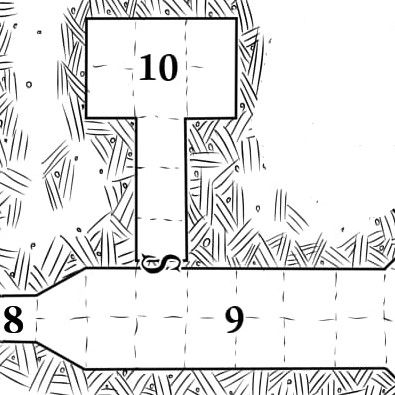
\includegraphics[width=\columnwidth]{pics/map_8-10.jpg}
\subsection{8 : Passage Secret}\label{n2:s8}
\begin{itemize}
  \item Directement sous \textbf{\nameref{n1:s7}}
  \item \'Etroite alcôve s’élargissant sur \textbf{\nameref{n2:s9}}
\end{itemize}

\subsection{9 : Hall aux Statues}\label{n2:s9}
Un long et large couloir.
\begin{itemize}
  \item Six énormes sculptures d’hommes-serpents en armes et armures
  \item Regard dédaigneux
  \item $1^{\`ere}$ à gauche : légèrement désalignée
  \item  déplacée, révèle \textbf{\nameref{n2:s10}}
\end{itemize}

\vfill\break
\subsection{10 : Salle de Garde Secrète}\label{n2:s10}
Cette pièce fut autrefois une salle de garde secrète pour
les assassins du temple.

\begin{itemize}
  \item Aujourd'hui vide et sombre.
  \item Les meubles ont pourri jusqu’à se désagréger.
  \item Deux guisarmes sont toujours utilisables
  \item Une icône religieuse en argent valant 50 PO.
\end{itemize}

\newpage
%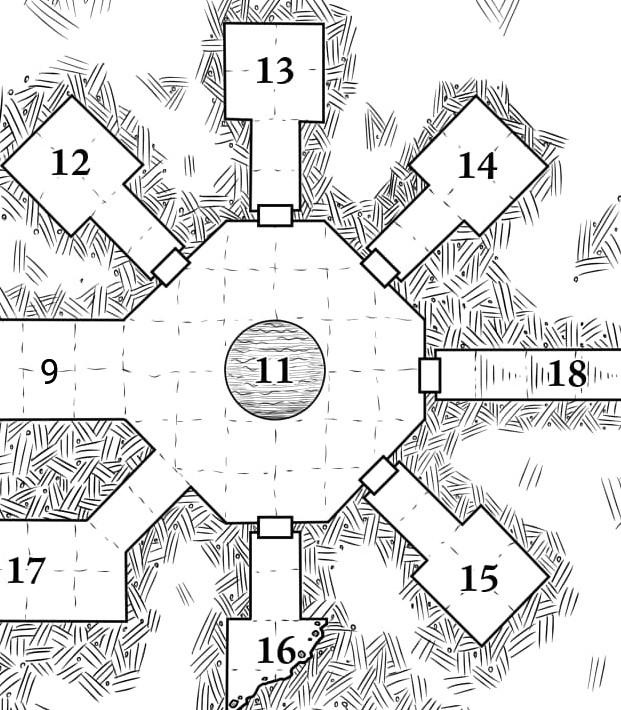
\includegraphics[width=\columnwidth]{pics/map_11-18.jpg}

\subsection{11 : Atrium des Tombes}\label{n2:s11}
\begin{itemize}
    \item Pièce octogonale, avec une ouverture au sud ouest, des portes sur les autres côtés
    \item Bordée de statues scrutatrices d’hommes-serpents
    \item Porte Sud-Est en bois
    \item Porte Est en pierre finement ouvragée: gravures de serpents pleuvant des cieux.
    \item Autres scellées par d’épaisses portes de pierre
    \begin{itemize}
        \item tombe aisément en faisant levier
    \end{itemize}
    \item Au centre fosse emplie d'eau
    \begin{itemize}
        \item Eau sombre et huileuse qui sent la réglisse
        \item Bassin profond de 3m
        \item 2 Fragments de Momie (Mains), bondissent et attaquent quiconque s’approche
    \end{itemize}
\end{itemize}

\begin{table}[h]
    \caption*{Fragments de Momie (Mains)}
    \begin{osetable}{X[2]X[1]X[1]X[2]}{0}
        CA          & 7 [12] & DV & 1* (4 pv) \\
        TACO        & 19 [0] & XP & 13 \\
        Attaque     & \SetCell[c=3]{l} 1D6 (griffes) & &\\
        Sauvegardes & \SetCell[c=3]{l} {\small MP~12 B~13 PP~14 S~15 SSB~16}& &\\
        Déplacement & 18m    & Moral & 12 \\
    \end{osetable}
\textbf{Maladie :}
\begin{itemize}
    \item Maladie putrescente au toucher
    \item Guérison magique inefficace
    \item Guérison naturelle 10x plus longue
    \item Ne peut être éliminée que par magie
\end{itemize}
\textbf{Mort-vivant}
\end{table}

Toucher l’eau ne déclenche pas de pourriture momifiante, mais la boire ou la mettre en contact avec une blessure ouverte, si.

Le bassin contient :
\begin{enumerate}
    \item Une tête de momie en furie qui a sombré depuis longtemps dans la folie ;
    \item Une lourde chaîne d’or valant 350 PO ;
    \item Un anneau magique en argent ;
    \item Un outil magique au choix du MJ ou aléatoire, ou 2d10x10 PO de joaillerie.
\end{enumerate}

\begin{highlight}[Anneau d’argent : bague de vision]
Enfilée au doigt, l’un des yeux du porteur jaillit de son orbite, et devient dur comme du verre.
L’\oe uil voit toujours normalement.
\end{highlight}

\subsection{12 : Tombe de Xisor le Vert}\label{n2:s12}
\subsubsection{Passage}
\begin{itemize}
    \item Dalle piégée dans le passage
    \item Active un sort d’éclair, vers l’entrée du couloir (4d6 dégâts, 2d6 si sauvegarde Sorts)
    \item Activé une seule fois
    \item Tiré depuis une plaque d’électrum dans le mur (100PO)
\end{itemize}
\subsubsection{Tombe}
Un parchemin de sort (venin oculaire, ou autre sort basé sur le venin) se trouve dans le
cercueil de Xisor.

\subsection{13 : Tombe de Sparamantur}\label{n2:s13}
\begin{itemize}
    \item Tombe est partiellement effondrée
    \item Si excavation : sons d'agitation de l'autre côté
    \item Sparamantur attaque à vue
    \item Ses ornements funéraires valent 100 PO
\end{itemize}

\begin{table}[ht]
    \caption*{Squelette homme-serpent (Sparamantur)}
    \begin{osetable}{X[2]X[1]X[1]X[2]}{0}
        CA          & 7 [12] & DV & 3 (13 pv) \\
        TACO        & 17 [2] & XP & 35 \\
        Attaque     & \SetCell[c=3]{l} 1D8 (Hache de bataille) & &\\
        Sauvegardes & \SetCell[c=3]{l} {\small MP~12 B~13 PP~14 S~15 SSB~16}& &\\
        Déplacement & 18m    & Moral & 12 \\
    \end{osetable}
\end{table}

\subsection{14 : Tombe de Franbinzar}\label{n2:s14}
\begin{itemize}
    \item Tombe décorée de peintures et gravures grossières
    \item Cercueil de pierre : restes de Franbinzar
    \item Ouverture : Franbinzar attaque (Pudding Noir)
    \item Trésor : copies d’argile, mais 20 PO d’anneaux sont noyés dans sa masse
\end{itemize}

\begin{table}[h]
    \caption*{Pudding Noir (Franbinzar)}
    \begin{osetable}{X[2]X[1]X[1]X[2]}{0}
        CA          & 6 [13] & DV & 5 (22 pv) \\
        TACO        & 15 [4] & XP & 300 \\
        Attaque     & \SetCell[c=3]{l} 2D8 (toucher) & &\\
        Sauvegardes & \SetCell[c=3]{l} {\small MP~10 B~11 PP~12 S~13 SSB~14}& &\\
        Déplacement & 18m    & Moral & 12 \\
    \end{osetable}
\begin{itemize}
    \item \textbf{Immunité :} Blessé uniquement par le feu
    \item \textbf{Division :} Les attaques qui ne sont pas liées au feu (y compris les sorts) provoquent la division du pudding. Chaque coup crée un nouveau pudding de 1 DV qui inflige 1d6 points de dégâts.
    \item \textbf{Corrosion :} Peut dissoudre le bois ou le métal en un tour.
    \item \textbf{Collant :} Peut se déplacer sur les murs et les plafonds.
    \item \textbf{Suintement :} Peut s’infiltrer à travers les petits trous et fissures.
    \item \textbf{Régénération :} Si tué, se régénère en 1d20 heures, à moins d’être incinéré.
\end{itemize}
Franbinzar était le dernier roi de la forteresse.

Sa momification ne s’est pas déroulée correctement.
Il s’est transformé en Pudding Noir.

On peut apercevoir 200PO d’anneaux noyés dans sa masse.
\end{table}
Si Franbinzar a été libéré, il est ajouté à la Table des Monstres Errants (p. 6) à la place d’un des présages.

\subsection{15 : Sacristie}\label{n2:s15}
Cette pièce était utilisée par les prêtres de la tombe supérieure.
Elle contient :
\begin{itemize}
    \item Trois lits,
    \item Des étagères vermoulues,
    \item Une icône religieuse de dieu-serpent en argent et émeraude (200 PO)
    \item Parchemins en langue inconnue (témoignent de la folie des momies emprisonnées).
          Éparpillés au sol.
\end{itemize}

\subsection{16 : Tombe Inachevée}\label{n2:s16}
Des outils d’excavation rouillent au sol.

\subsection{17 : Soldats d’Argile}\label{n2:s17}
\begin{itemize}
    \item 3 rang de 6 statues d’argile de soldats hommes-serpents à taille réelle
    \item Leurs épées sont rouillées et inutiles
    \item Creuses mais vides
    \item Celle au coin sud-ouest cache un passage secret vers 38 : le Hall du Basilic (p. 9)
\end{itemize}

\newpage
%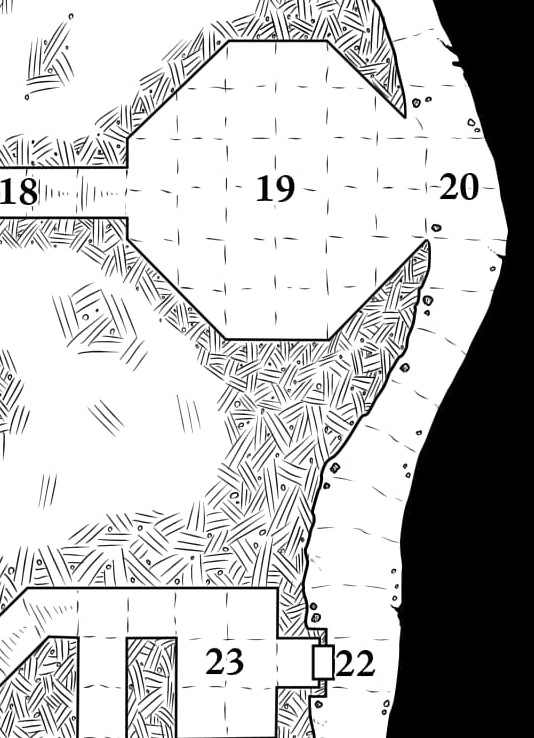
\includegraphics[width=\columnwidth]{pics/map_18-23.jpg}

\subsection{18 : Escaliers}\label{n2:s18}
\begin{itemize}
    \item Des escaliers s’enfoncent dans les ténèbres.
    \item Une légère brise se fait sentir.
\end{itemize}

La troisième volée de marches est piégée.

\begin{highlight}[Piège]
Dès qu’un poids est appliqué sur la marche
\begin{itemize}
    \item Les marches basculent pour former une rampe de roche lisse
    \item Des épieux jaillissent du sol en bas de l’escalier (1D8 dégâts, 1D4 si sauvegarde Mort)
    \item Se réarme après 5 rounds
\end{itemize}
\end{highlight}

\subsection{19 : Arène du Gardien Cobra}\label{n2:s19}
\begin{itemize}
    \item Même forme et taille que \nameref{n2:s11}
    \item Arène tapissée de boucliers divers (des tribus vaincues par les hommes-serpents)
    \item 5 sont fonctionnels, les autres pourris
    \item 20 PO récupérables en les désassemblant (décorations en argent)
    \item Au centre une statue de pierre en forme de cobra
\end{itemize}

\begin{table}[h]
    \caption*{Gardien Cobra de Pierre}
    \begin{osetable}{X[2]X[1]X[1]X[2]}{0}
        CA          & 6 [13] & DV & 5 (22 pv) \\
        TACO        & 15 [4] & XP & 300 \\
        Attaque     & \SetCell[c=3]{l} 2D8 (toucher) & &\\
        Sauvegardes & \SetCell[c=3]{l} {\small MP~10 B~11 PP~12 S~13 SSB~14}& &\\
        Déplacement & 18m    & Moral & 12 \\
    \end{osetable}
\end{table}